\graphicspath{{./figures/}}
\chapter{Methodology} 
The following chapter provides an overview over the relevant development 
components that are used within this project.
Therefore, the used software packages are introduced before a short outline of
the utilized drone hardware is given.

\section{Software fundamentals}
\label{sec:2_software_fund}
As the main part of this project's software will run on a portable remote 
computer allowing for not only to control the drone but also to perform the 
long jump analysis on video inputs, every software component is chosen to 
demand as little hardware requirements as possible.
Especially no \ac{GPU} is required to run the software.
All image processing is performed using the \ac{CPU} only.
Furthermore, the software is designed to run platform independent.\\

\subsection{Programming Language and why Python}
\label{subsec:2_programming_language}
Python is the most used programming language in the scientific area.

\subsection{Mediapipe for detecting body poses}
\label{subsec:2_mediapipe_framework}
One of the software's main tasks is to perform a human body pose detection on
video inputs.
Because this part runs on the remote computer only, it can also handle
pre-recorded videos that should be evaluated.\\
The evaluation itself is performed using the mediapipe framework.
This framework uses a pre-trained convolutional neural network that is able to
detect 33 key points in human body poses \cite{mediapipe_paper}.
The network could theoretically even be fine-tuned to improve its accuracy on
specific input types.
Even if this so called \textit{transfer-training} method requires significantly
less training data than training a neural network from scratch, it is not applied
within this project as first test runs already showed reliable results.\\
Furthermore, the mediapipe framework does not require any hardware acceleration
and is renowned for its precise output.
Hii et al.~for example showed in~\cite{mp_gait_analysis}, 
\cite{mp_gait_analysis_2} that the framework can be applied in medical gait 
analysis applications to replace marker based approaches.\\
Moreover, Mediapipe offers three different detection models that differ in 
terms of speed and accuracy.
The fastest detection model offers the lowest accuracy and vice versa.\\
Additionally, Mediapipe is optimized for multiple input types including videos 
and live streams, which is ideal for this project.\\
\autoref{fig:2_body_keypoints} shows an overview of the 33 detectable key 
points. 
\begin{figure}[!h]
    \centering
    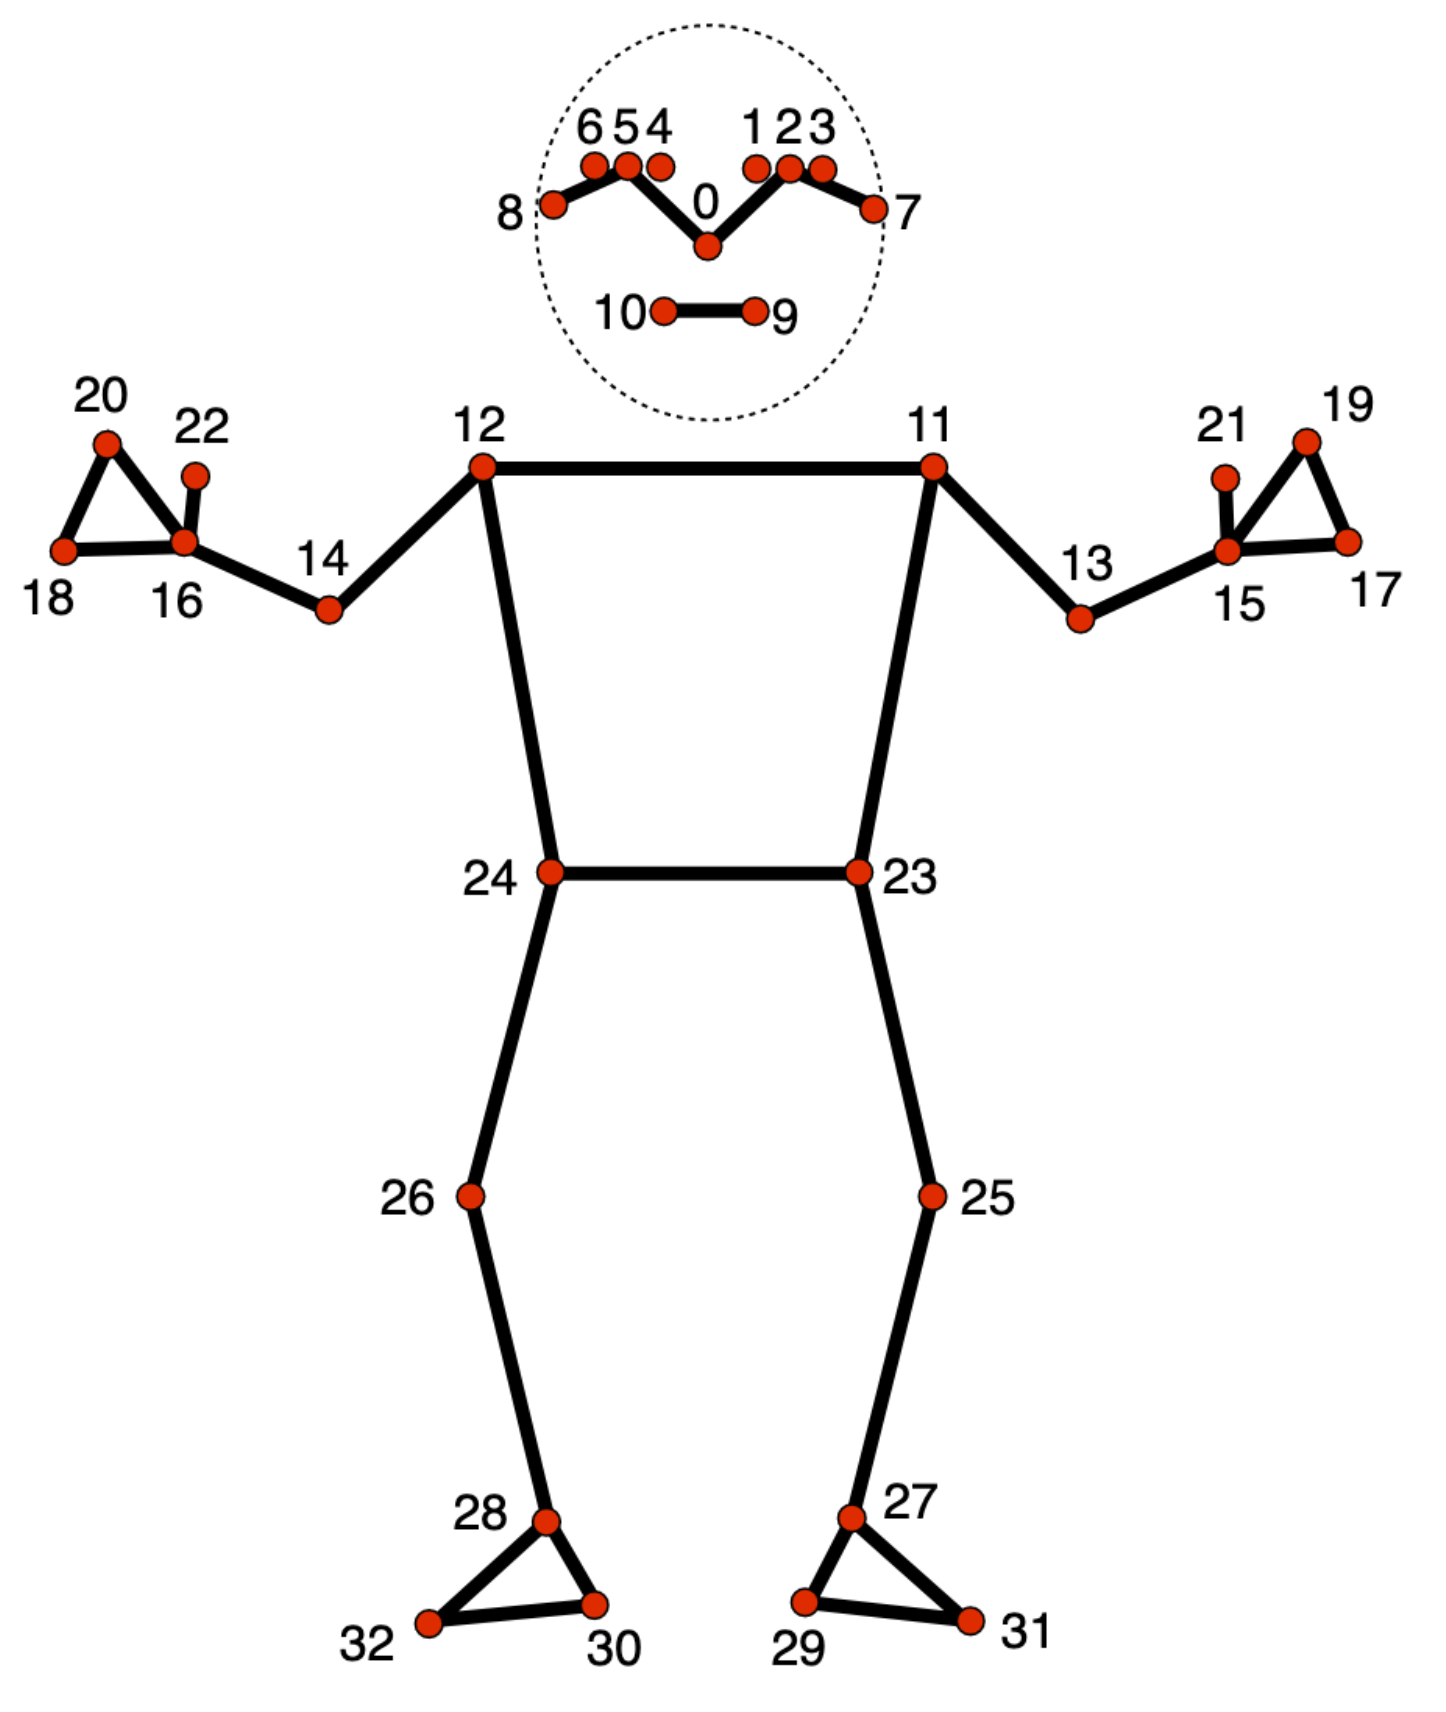
\includegraphics[scale=0.3]{figures/body_key_points.png}
    \caption[Set of detectable body key points]
    {Fixed set of detectable body key points offered by the mediapipe framework
    \cite{mediapipe_framework}}
    \label{fig:2_body_keypoints}
\end{figure}\\
Within this work, the key points in the head area (range [0 - 10]) are not of 
great interest apart from visualization purposes.\\
The knee, hip and arm key points however will be used for angle 
calculations and ground contact detection.
Thus, a good performance in detecting the according key points within these 
areas is crucial for the software's overall reliability.

\subsection{Why Mediapipe?}
In recent years many approaches towards accurate body pose detection were 
developed and implemented.
Many of those offer decent accuracies, but often lack reasonable performance,
especially when no \ac{GPU} is available for hardware acceleration.
Following two common alternatives to Mediapipe, namely OpenPose and AlphaPose,
are shortly presented and differentiated from the chosen Mediapipe framework.\\
One of the most widely used human pose detection libraries is the open source 
library \textit{OpenPose}.
As shown in~\cite{openPose} it offers a Multi-Person pose estimation that is 
especially useful when dealing with groups of people.
However, as this project is meant to be used for long jump evaluation, only one 
person needs to be tracked at a time.
Even though OpenPose of course can handle one person pose estimation, 
mediapipe outperforms OpenPose in this area.
Back in 2016 Kocabas et al.~achieved around 23~FPS using \ac{GPU} accelerated
OpenPose pose detection \cite{openPose_speed_gpu} and Osokin later proposed an
improved neural network design, allowing for up to 28~FPS without hardware 
acceleration \cite{openPose_speed_cpu}.
As of 2023 these benchmarks are still reasonable.
Mediapipe however achieves speeds of up to 63\% higher.\\
While OpenPose uses a \textit{Bottom-Up} approach due its multi-person 
application, Mediapipe uses the less computational complex \textit{Top-Down} 
approach.\\
Bottom-Up implementations first detect all body key points present in an input
image and then move on to grouping the recognized points in clusters.
Points in the same cluster are then assigned to one person.\\
Top-Down approaches however first roughly detect the overall body position 
within the input image and then define a region of interest\footnote{sometimes
also referred to as \textit{Bounding Box}} around the subject.
The following processing therefore only needs to take this defined region of 
interest into account, leading to significantly less computational complexity.\\
AlphaPose is another open source library often used for body pose estimation.
Just like OpenPose it uses a Bottom-Up approach to reliable offer multi-person
body pose detection.
Additionally, AlphaPose, like Mediapipe, offers multiple detection models that 
differ regarding accuracy and speed.
Again however, Mediapipe outperforms AlphaPose because of its Top-Down approach
and because AlphaPose is designed to work with \ac{GPU} acceleration, rather 
than running on \ac{CPU} only.\\
Another advantage of Mediapipe is its output.
While OpenPose and AlphaPose offer 2D coordinates for each detected key point,
Mediapipe additionally offers a depth estimation resulting in a spatial 3D 
coordinate for each detected key point.
Thereby, more comprehensive analysis can be performed.   
